\documentclass{llncs}
\usepackage{makeidx}
\usepackage{amsmath}
\usepackage{amsfonts}
\usepackage{amssymb}
\usepackage[spanish]{babel}
\usepackage{graphicx}

%opening
\title{\large\huge Super Proyecto\\de \\ IA + Compilación + Simulación}
\author{Integrantes: \\ Julio José Horta C312 \\Javier Villar Alonso C311 \\ Dayron Fernández C311}

\begin{document}
	
\maketitle

\newpage

\section{General}
En este trabajo se tiene como objetivo simular el desarrollo de la vida en cualquier planeta y acercarnos lo más posible a la forma adaptativa de las especies ante los cambios naturales, la evolución de la misma y la competencia entre estas tal cual como ocurren en nuestro mundo natural, con objetivo reunir datos estadísticos del comportamiento natural de las especies para asi asimilar mejor su expansión natural y adaptabilidad en el mundo, asi como que tan dañino pueda ser un fenómeno en específico. 

\section{Aplicación}
El proyecto cuenta con una aplicación que permite poder modificar parámetros de la simulación para poder crear una interacción en un mundo donde se desea manifestar el comportamiento de la vida y ver resultados atendiendo al número de ocurrencia de acciones, cantidad de individuos nacidos, cantidad de muertes, entre otras.

\section{Simulación}

\subsection{Mapa}
El mapa es el mundo en el que se llevará a cabo la simulación. Este mundo consta de una matriz donde establecemos el tamaño de nuestro mapa de acuerdo al largo y ancho, a lo cual nombramos tamaño del eje X y tamaño del eje Y respectivamente, además de mandar la cantidad de zonas que serán creadas genéricamente para el mundo que queremos simular
\newline
\newline
Para recorrer el mapa usaremos una matriz adecuada a los tamaños mandados, en el que cada una de las coordenadas es un Tile (la cual estaremos explicando posteriormente). También se llevarán como variable cada una de las zonas existentes en el mundo de forma independientes aunque sean del mismo tipo
\newline
\newline
Este mapa está diseñado para que no existan límites ya que tiene más sentido para nuestra simulación que sea un entorno circular antes que cuadrático

\subsection{Zones}
Una zona es un ambiente natural que consta de un conjunto de tiles que expresan la expansión en la que vivirán nuestras especies.
\newline
\newline
Estas constan de una variable Tiles que agrupará en un array todos los tiles que corresponden a la zona, un string que exprese el tipo de zona, una variable danger que proporcionará cuán peligroso es la zona, y por último un contador de cuántos tiles hay en la zona


\subsection{Tiles}
Un tile es una ubicación de una zona natural del mapa en el que los individuos de las diferentes especies interactúan en ella, ya sea en busca de alimentos, de compañeros de una especie o la caza de estos para alimentarse. Es importante aclarar que un tile no tiene límite de tamaño, sino que está definida para que varios individuos puedan convivir en ella y posible existencia de abundantes recursos y componentes
\newline
\newline
Estos tiles constan de las coordenadas de ubicación de la zona, las cantidad de criaturas que se encuentran en ella, los recursos disponibles en ella guardados en una variable llamada ComponentsDict

\section{Especies}
Para poder crear una interacción en el mundo creado decidimos añadir especies para que formen parte de este mundo. Estas especies presentarán unas características generales por donde rondaran las estadísticas del grupo de individuos de esta especie.
\newline
\newline
Este recibe un número que especifica la cantidad de individuos que se quiere para añadirlos en una posición determinada en el mapa, para eso se debe mandar las coordenadas en donde se quiere ubicar. 


\subsection{Evolución}
Una especie tiene la capacidad de evolucionar en una nueva, tomando características promedio de los individuos de la especie padre en una zona determinada y modificando algunas otras características como tipo de alimentación, canibalismo, cantidad de células, entre otras

\section{Agentes Inteligentes}
Un agente inteligente, es una entidad capaz de percibir su entorno, procesar tales percepciones y responder o actuar en su entorno de manera racional, es decir, de manera correcta y tendiendo a maximizar un resultado esperado. Es capaz de percibir su medio ambiente con la ayuda de sensores y actuar en ese medio utilizando elementos que reaccionan a un estímulo realizando una acción.
\newline
\newline
Bajo este concepto se desarrolló la entidad de los individuos 


\section{Individuos}
Los individuos son las formas de vida de una especie que interactúan y realizan funciones básicas para vivir en el mundo definido. Esta interacción la lleva a cabo en unas coordenadas del mapa en el que andamos trabajando donde estarán en constante interacción con el medio (tile)

\subsection{Reproducción}
Cada individuo posee un tipo de reproducción que bajo esta condición se puede conocer si un individuo tiene reproducción sexual o asexual para poder llevar a cabo probabilísticamente la aparición de un nuevo individuo mediante el conocimiento de un individuo femenino fértil con el que llevar a cabo la reproducción, o en el caso de los asexuales, realizar una clonación del individuo al que queremos llevar a cabo una reproducción
\newline
\newline
Para simular esta reproducción usamos el método Breed

\subsection{Movimiento del individuo}
Cada individuo puede moverse de acuerdo a una velocidad traducida en la cantidad
de casillas del recorrido, este se moverá de acuerdo a la inteligencia del individuo, la cual definirá cuantos criterios valorará para moverse.
\newline
\newline
Los criterios son los siguientes:

\begin{enumerate}
	\item Buscar comida
	\item Buscar peligro
	\item Buscar manada
	\item Buscar pareja
\end{enumerate}

Estos criterios son mandados en pequeñas matrices que simularan el mapa de percepción del individuo, donde las zonas de mayor interés de conocimiento de este estarán evaluados en 1 y una vez definido cuales son los criterios que valorará de acuerdo a la inteligencia del individuo, serán sumadas las matrices para tener así una matriz pesada que poder usar para proceder al movimiento A* del individuo (UcsSmart).
\newline
\newline
Este A* es realizado usando un mapa perceptivo donde procederemos a trabajar el movimiento del individuo, en el que empezamos a atribuir aristas pesadas de movimiento que después serán revisadas en orden de prioridad de acuerdo a la heurística de distancia Euclidiana.Todas las casillas están pesadas entre 1 y 5, el camino más cercano de una casilla a otra solo puede ser 1 por lo que nuestra heurística Euclidiana es optimista ya que no habrá camino más corto que la línea recta.
\newline
\newline
Una vez terminado de aristas los caminos, hasta llegar al destino, obtendremos un grafo ponderado del se tendría el camino mediante el recorrido entre padres en el grafo.
\newline
\newline
Luego este método funcionará como un drijktra, un método estudiado en estructura
de datos para determinar la longitud del camino más corto entre dos vértices de
un grafo ponderado simple, conexo y no dirigido con n vértices. Luego de tener el camino correcto llamaremos al método fixroad que se encarga de ir regresando desde el nodo final hasta el inicial por los padres para saber el camino a tomar para así tener el camino por donde recorrerá el individuo, donde por cada posición en que se mueva comprobamos si, bajo la probabilidad de morir al moverse, el individuo termina muriéndose en ese tile o termina llegando a destino luego de la comprobación en el destino.


\subsection{Situación de Combate}
En este proyecto se implementó la posibilidad en que dos individuos terminen en un encuentro de combate entre ambos. Estos terminan surgiendo en la necesidad de que una especie canibal decida alimentarse de otro individuo del mundo con el que está interactuando. Esta situación se producirá en un mapa de tamaño 10*velocidad máxima entre los dos individuos y existen dos fases en el encuentro: 

\begin{enumerate}
	\item \textbf{Fase de Acercamiento}: viene dado en un momento de tranquilidad donde el individuo cazador se acerca con sigilo a la presa de la que se desea alimentar.
	\item \textbf{Fase de Combate}: viene dado en el momento que ambos llegan a percibirse, ya sea porque terminó siendo descubierto el cazador o la presa recibiendo el golpe
\end{enumerate}

Para llevar a cabo el combate se llevará a cabo en un sistema por turno y se usará un Min-max donde llevaremos unos diccionarios de registros llamados battlelog para cada individuos donde registraremos la vida, lenteos, daños y otros elementos. Una vez seteados los elementos del battlelog necesarios para llevar el combate es que empezamos a reproducir esta situación


\subsubsection{Fase de Acercamiento}
Una vez comienza el combate empieza la fase de acercamiento, esta radica en que el cazador se irá acercando casilla a casilla hacia la presa mediante un método llamado sneakwalk que recibe el sigilo del cazador y se lleva contra la inteligencia y percepción de la presa promediada, mientras mayor sea el sigilo del cazador comparado con el promedio de percepción e inteligencia de la presa, menos posibilidades tendrá de ser descubierto el cazador. Esta probabilidad se realizará mediante una distribución normal entre ambos datos y en caso que el cazador alcance al objetivo, la presa recibirá un golpe de mucho daño.
\newline
\newline
En dependencia de quien inicia el combate, se llamará al turno del cazador o la presa para iniciar el combate.

\subsubsection{Fase de Combate}
La fase de combate radica en que se irán turnando la presa y el individuo por turno con el sistema en que la presa intentará esquinarse de forma tal que esté huyendo del cazador y el cazador se acerque lo más que pueda a la presa para poder realizar su ataque. En esos sistemas consisten las heurísticas de la presa y el cazador, respectivamente.
\newline
\newline
En esta fase de combate no existe una cantidad máxima de turnos de duración, este llegará a su final si la presa logra esquinarse al borde del mapa de combate o el cazador logra eliminar a la presa.
\newline
\newline
Si el cazador llega a estar a una casilla de diferencia de la presa, el cazador llegará a realizar un golpe a la presa de los siguientes que se encuentran a disposición:

\begin{enumerate}
	\item Golpe normal: golpe que realiza una cantidad de daño delimitada en las estadísticas del individuo
	\item Golpe crítico: golpe fuerte tiene probabilidad de que haga menos daño pero existe gran probabilidad que haga más daño que el golpe normal
	\item Golpe de lenteo: golpe que se caracteriza en disminuir la velocidad de los contrincantes
\end{enumerate}

Si el cazador logra eliminar a la presa en el combate, este satisfacerá su saciedad al alimentarse de él

\section{Anexos}
     
\begin{figure}
	\centering
	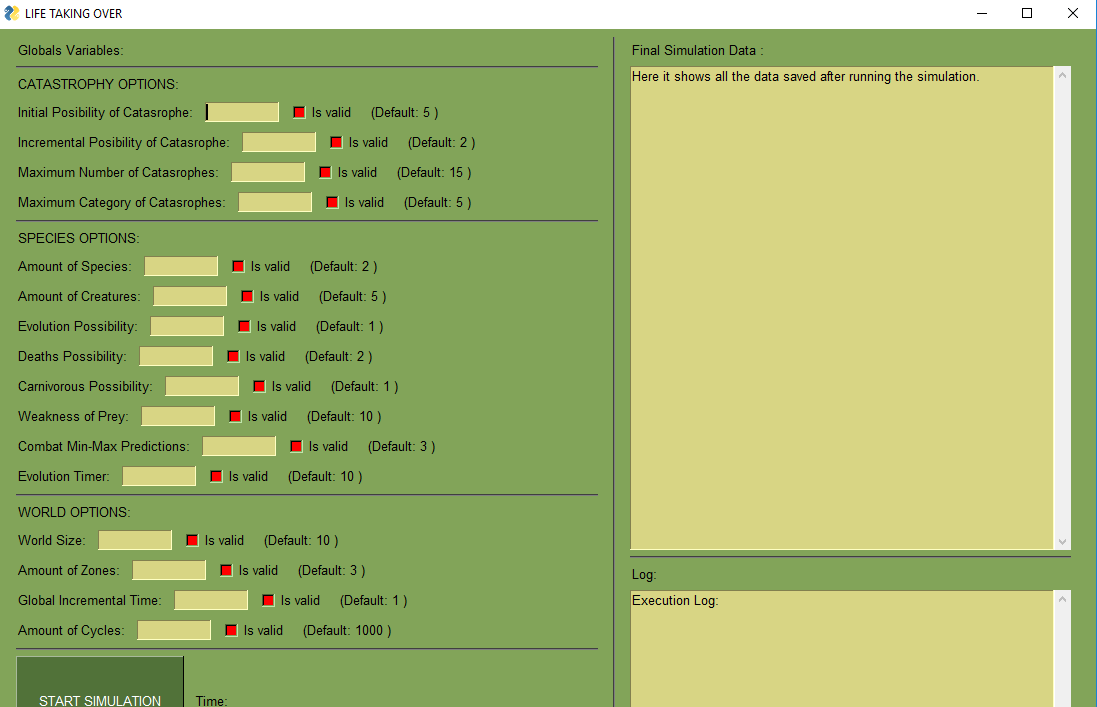
\includegraphics[width=1.0\linewidth]{imagenesapk/HomeForm}
	\label{fig:homeform}
\end{figure}

\begin{figure}
	\centering
	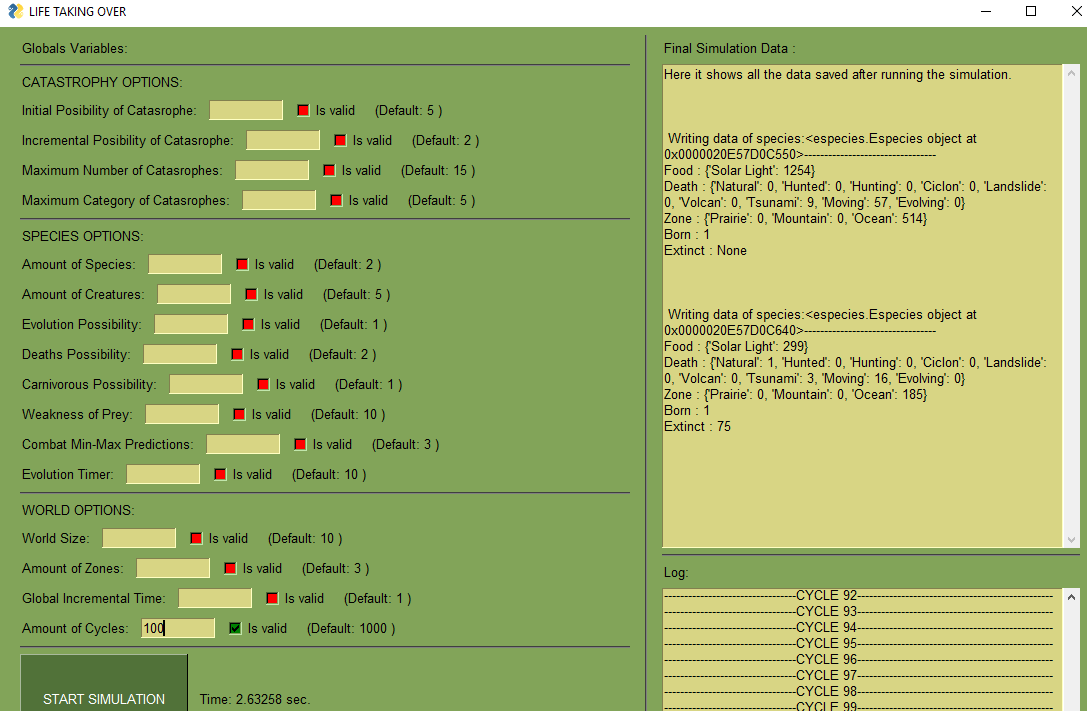
\includegraphics[width=1.0\linewidth]{imagenesapk/ResultForm}
	\label{fig:resultform}
\end{figure}

\end{document}
